\section{Wstęp}

W ramach projektu z przedmiotu "Wstęp do Robotyki" mieliśmy za zadanie wykonać robota śledzącego linie oraz przenoszącego ładunek. W ciągu 6 spotkań laboratoryjnych zbudowaliśmy fizyczną konstrukcję oraz stworzyliśmy oprogramowanie do jego obsługi.

\section{Konstrukcja}

Główny element konstrukcji to kostka odpowiedzialna za funkcjonalność całego robota.

\begin{figure}[H]
    \centering
    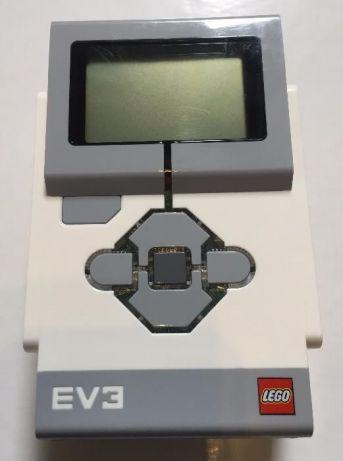
\includegraphics[width=0.4\textwidth]{Images/main}
    \caption[]{Kostka}
\end{figure} 

Pierwszy pomysł na konstrukcję robota zakładał użycie jednego silnika do napędu oraz drugiego sterującego osią skrętną.Po kilku próbach okazało się że robot miał duże problemy ze skręcaniem, a do tego wysoka konstrukcja negatywnie wpływała na stabilność.\\
Przy drugiej próbie wykonaliśmy bardziej standardową konstrukcję z użyciem dwóch dużych silników do napędu dwóch kół oraz kulki jako trzeciego punktu podparcia z tyłu.\\
Do podnoszenia paczki zamontowaliśmy średni silnik z obrotowym hakiem do zaczepienia paczki. 

\begin{figure}[H]
    \centering
    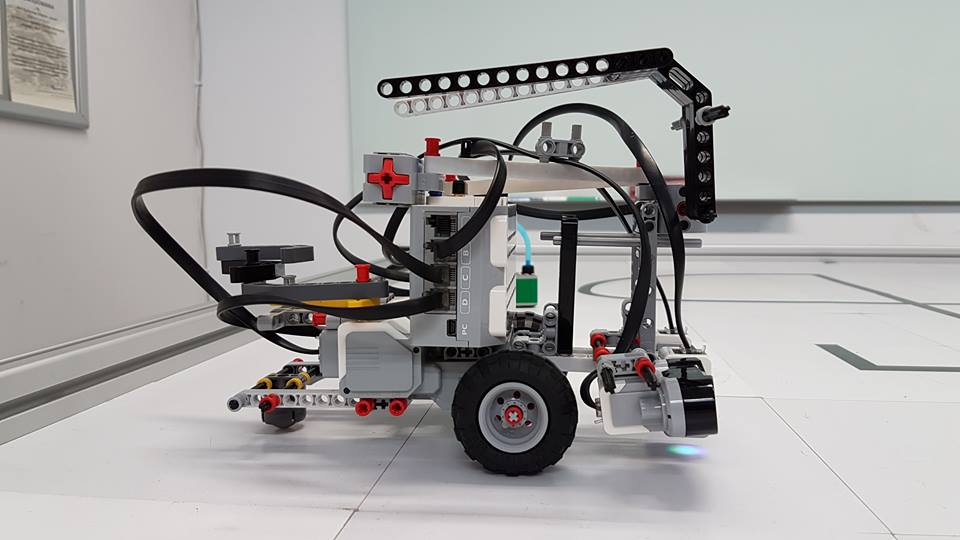
\includegraphics[width=0.8\textwidth]{Images/structure}
    \caption[]{Konstrukcja}
\end{figure} 

Po jakimś czasie dodaliśmy także guzik do wyłączania programu dla ułatwienia testów.

\begin{figure}[H]
    \centering
    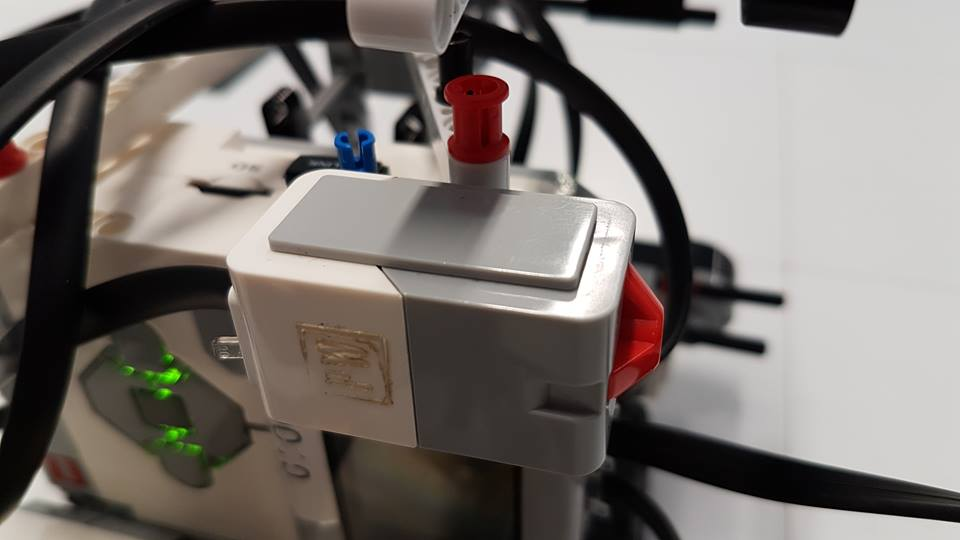
\includegraphics[width=0.8\textwidth]{Images/touch_sensor}
    \caption[]{Czujnik dotyku}
\end{figure}

W celu wykrywania linii zamontowaliśmy na przodzie robota dwa czujniki światła które miały wykrywać kolor czarny i w takim wypadku skręcać w odpowiednim kierunku. Początkowo były one umieszczone zbyt wysoko, ale po opuszczeniu osiągnęliśmy oczekiwany rezultat.

\begin{figure}[H]
    \centering
    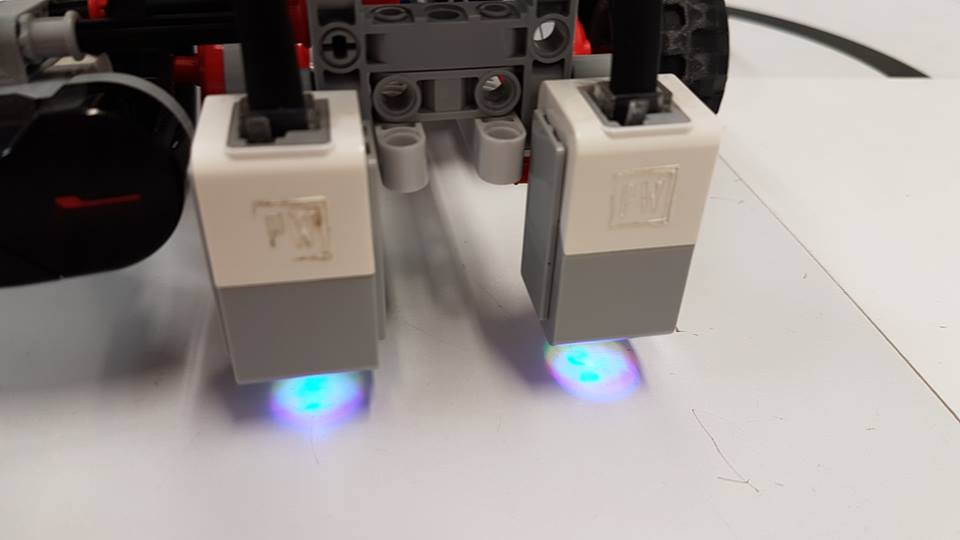
\includegraphics[width=0.8\textwidth]{Images/light_sensors}
    \caption[]{Czujniki światła}
\end{figure}

Obok czujników światła znajduje się czujnik podczerwieni służący do wykrywania ładunku do przetransportowania.

\begin{figure}[H]
    \centering
    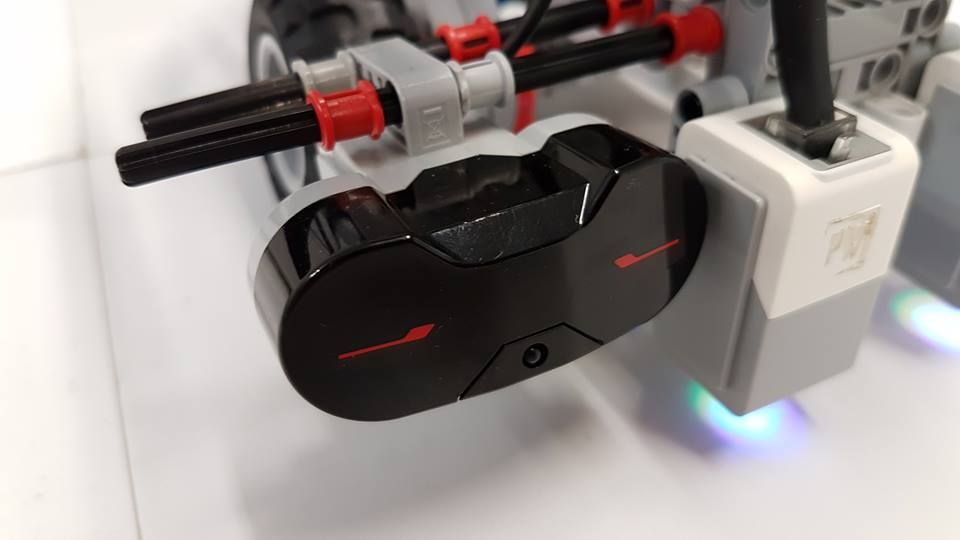
\includegraphics[width=0.8\textwidth]{Images/infrared_sensor}
    \caption[]{Czujnik podczerwieni}
\end{figure}

\section{Oprogramowanie}

W zaprojektowanym oprogramowaniu użyliśmy szeregu funkcji:
\begin{itemize}
\item
\textit{calibrate} w celu odpowiedniej kalibracji czujników światła,
\item
\textit{colorSum} oraz \textit{countTheta}, gdzie pierwsza z nich wyznacza sumę wszystkich zmiennych RGB z danego czujnika światła, a druga dokonuje zmiany składowych RGB na pseudoHSV,
 \item
 \textit{checkRed/checkGreen} zwracające prawdę jeżeli czujnik światła w danym momencie znajduje się nad kolorem czerwonym/zielonym, 
 \item
 \textit{dropBlock/pickUp} służące do opuszczania/podnoszenia ładunku,
 \item
\textit{returnToLine} wykorzystanej przy podnoszeniu i opuszczaniu ładunku, w celu powrotu na linię po wykonaniu zadania,
 \item
 \textit{run} oraz \textit{steering} realizujące główną funkcjonalność z użyciem algorytmu PID
\end{itemize}

\begin{figure}[H]
    \centering
    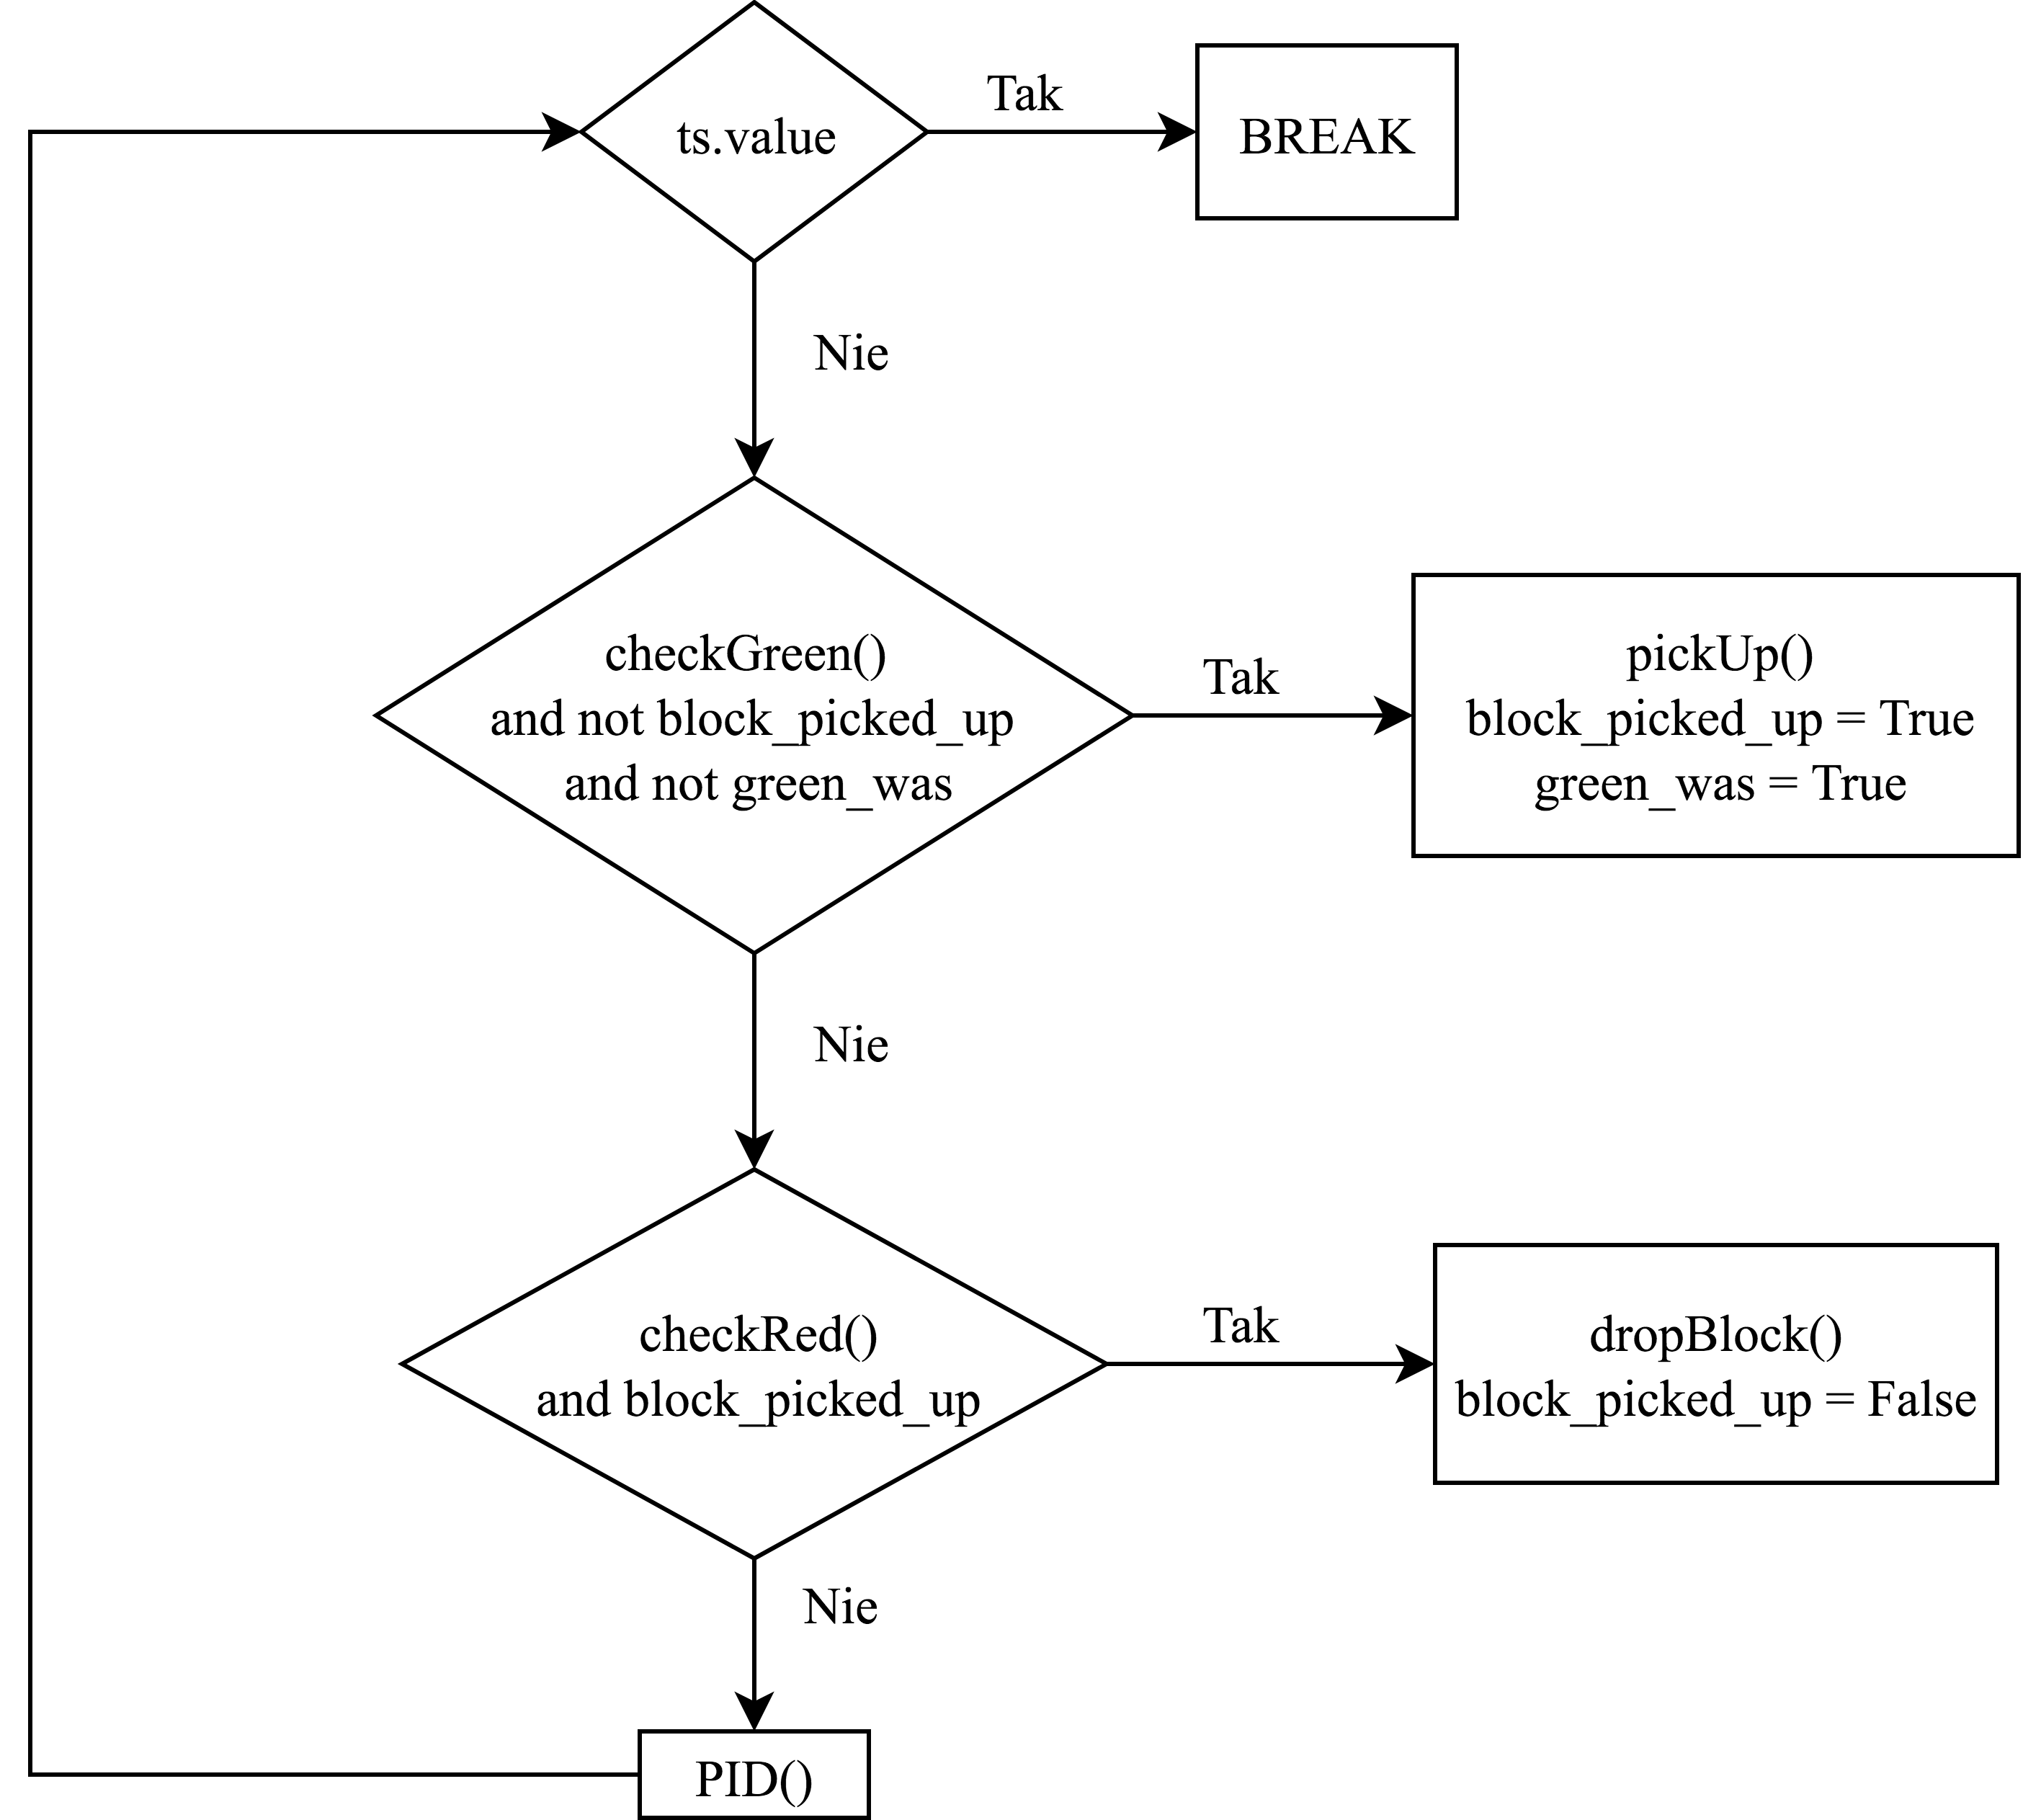
\includegraphics[width=0.8\textwidth]{Images/Cargo}
    \caption[]{Algorytm przenoszenia ładunku}
\end{figure}

\begin{figure}[H]
    \centering
    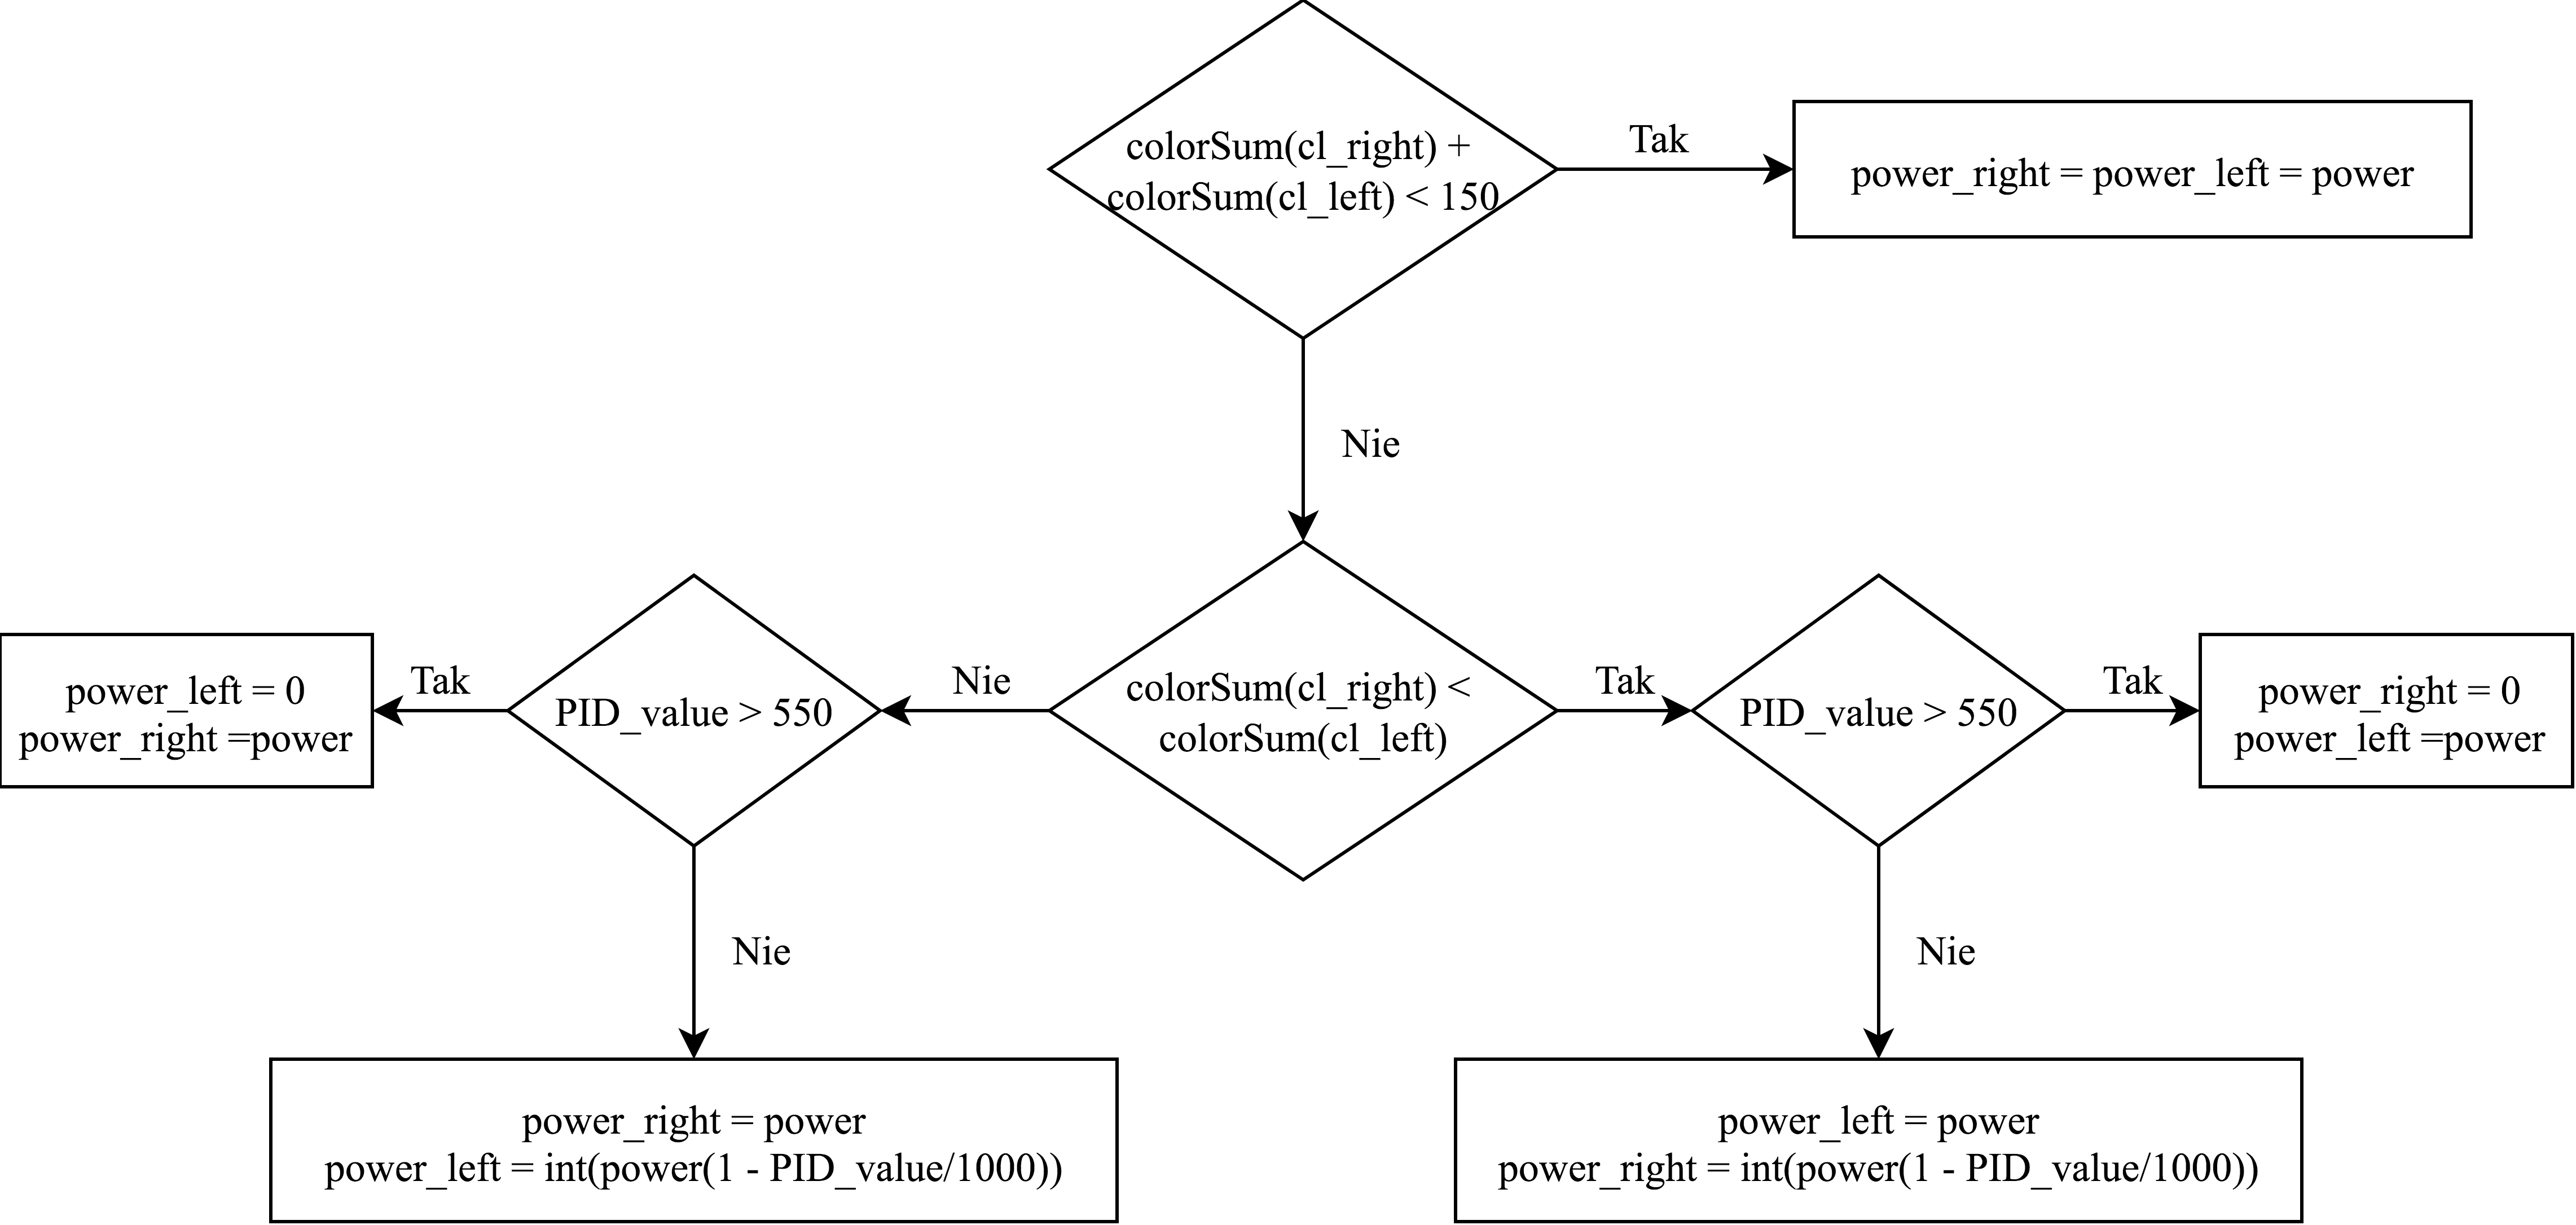
\includegraphics[width=1.2\textwidth]{Images/Sterring}
    \caption[]{Algorytm sterowania}
\end{figure}